

\documentclass[letterpaper,11pt]{article}
\newlength{\outerbordwidth}
\pagestyle{empty}
\raggedbottom
\raggedright
\usepackage[svgnames]{xcolor}
\usepackage{framed}
\usepackage{tocloft}
\usepackage{graphicx}
\usepackage{times}
\usepackage{multirow}
\usepackage[utf8]{inputenc}
\usepackage{tabularx}

%-----------------------------------------------------------

\setlength{\outerbordwidth}{3pt}  % Width of border outside of title bars
\definecolor{shadecolor}{gray}{0.75}  % Outer background color of title bars (0 = black, 1 = white)
\definecolor{shadecolorB}{gray}{0.93}  % Inner background color of title bars


%-----------------------------------------------------------

\setlength{\evensidemargin}{-0.25in}
\setlength{\headheight}{0in}
\setlength{\headsep}{0in}
\setlength{\oddsidemargin}{-0.25in}
\setlength{\paperheight}{11in}
\setlength{\paperwidth}{8.5in}
\setlength{\tabcolsep}{0in}
\setlength{\textheight}{9.5in}
\setlength{\textwidth}{7in}
\setlength{\topmargin}{-0.3in}
\setlength{\topskip}{0in}
\setlength{\voffset}{0.1in}


%-----------------------------------------------------------
%Custom commands
\newcommand{\resitem}[1]{\item #1 \vspace{-2pt}}
\newcommand{\resheading}[1]{\vspace{5pt}
  \parbox{\textwidth}{\setlength{\FrameSep}{\outerbordwidth}
    \begin{shaded}
\setlength{\fboxsep}{0pt}\framebox[\textwidth][l]{\setlength{\fboxsep}{4pt}\fcolorbox{shadecolorB}{shadecolorB}{\textbf{\sffamily{\mbox{~}\makebox[6.762in][l]{\large #1} \vphantom{p\^{E}}}}}}
    \end{shaded}
  }\vspace{-5pt}
}
\newcommand{\ressubheading}[4]{
\begin{tabular*}{6.5in}{l@{\cftdotfill{\cftsecdotsep}\extracolsep{\fill}}r}
		\textbf{#1} & #2 \\
		\textit{#3} & \textit{#4} \\
\end{tabular*}\vspace{-6pt}}
%-----------------------------------------------------------

\begin{document}

%-----------------------------------------------------------

\begin{tabular*}{7in}{l@{\extracolsep{\fill}}r}
  & \multirow{4}{*}{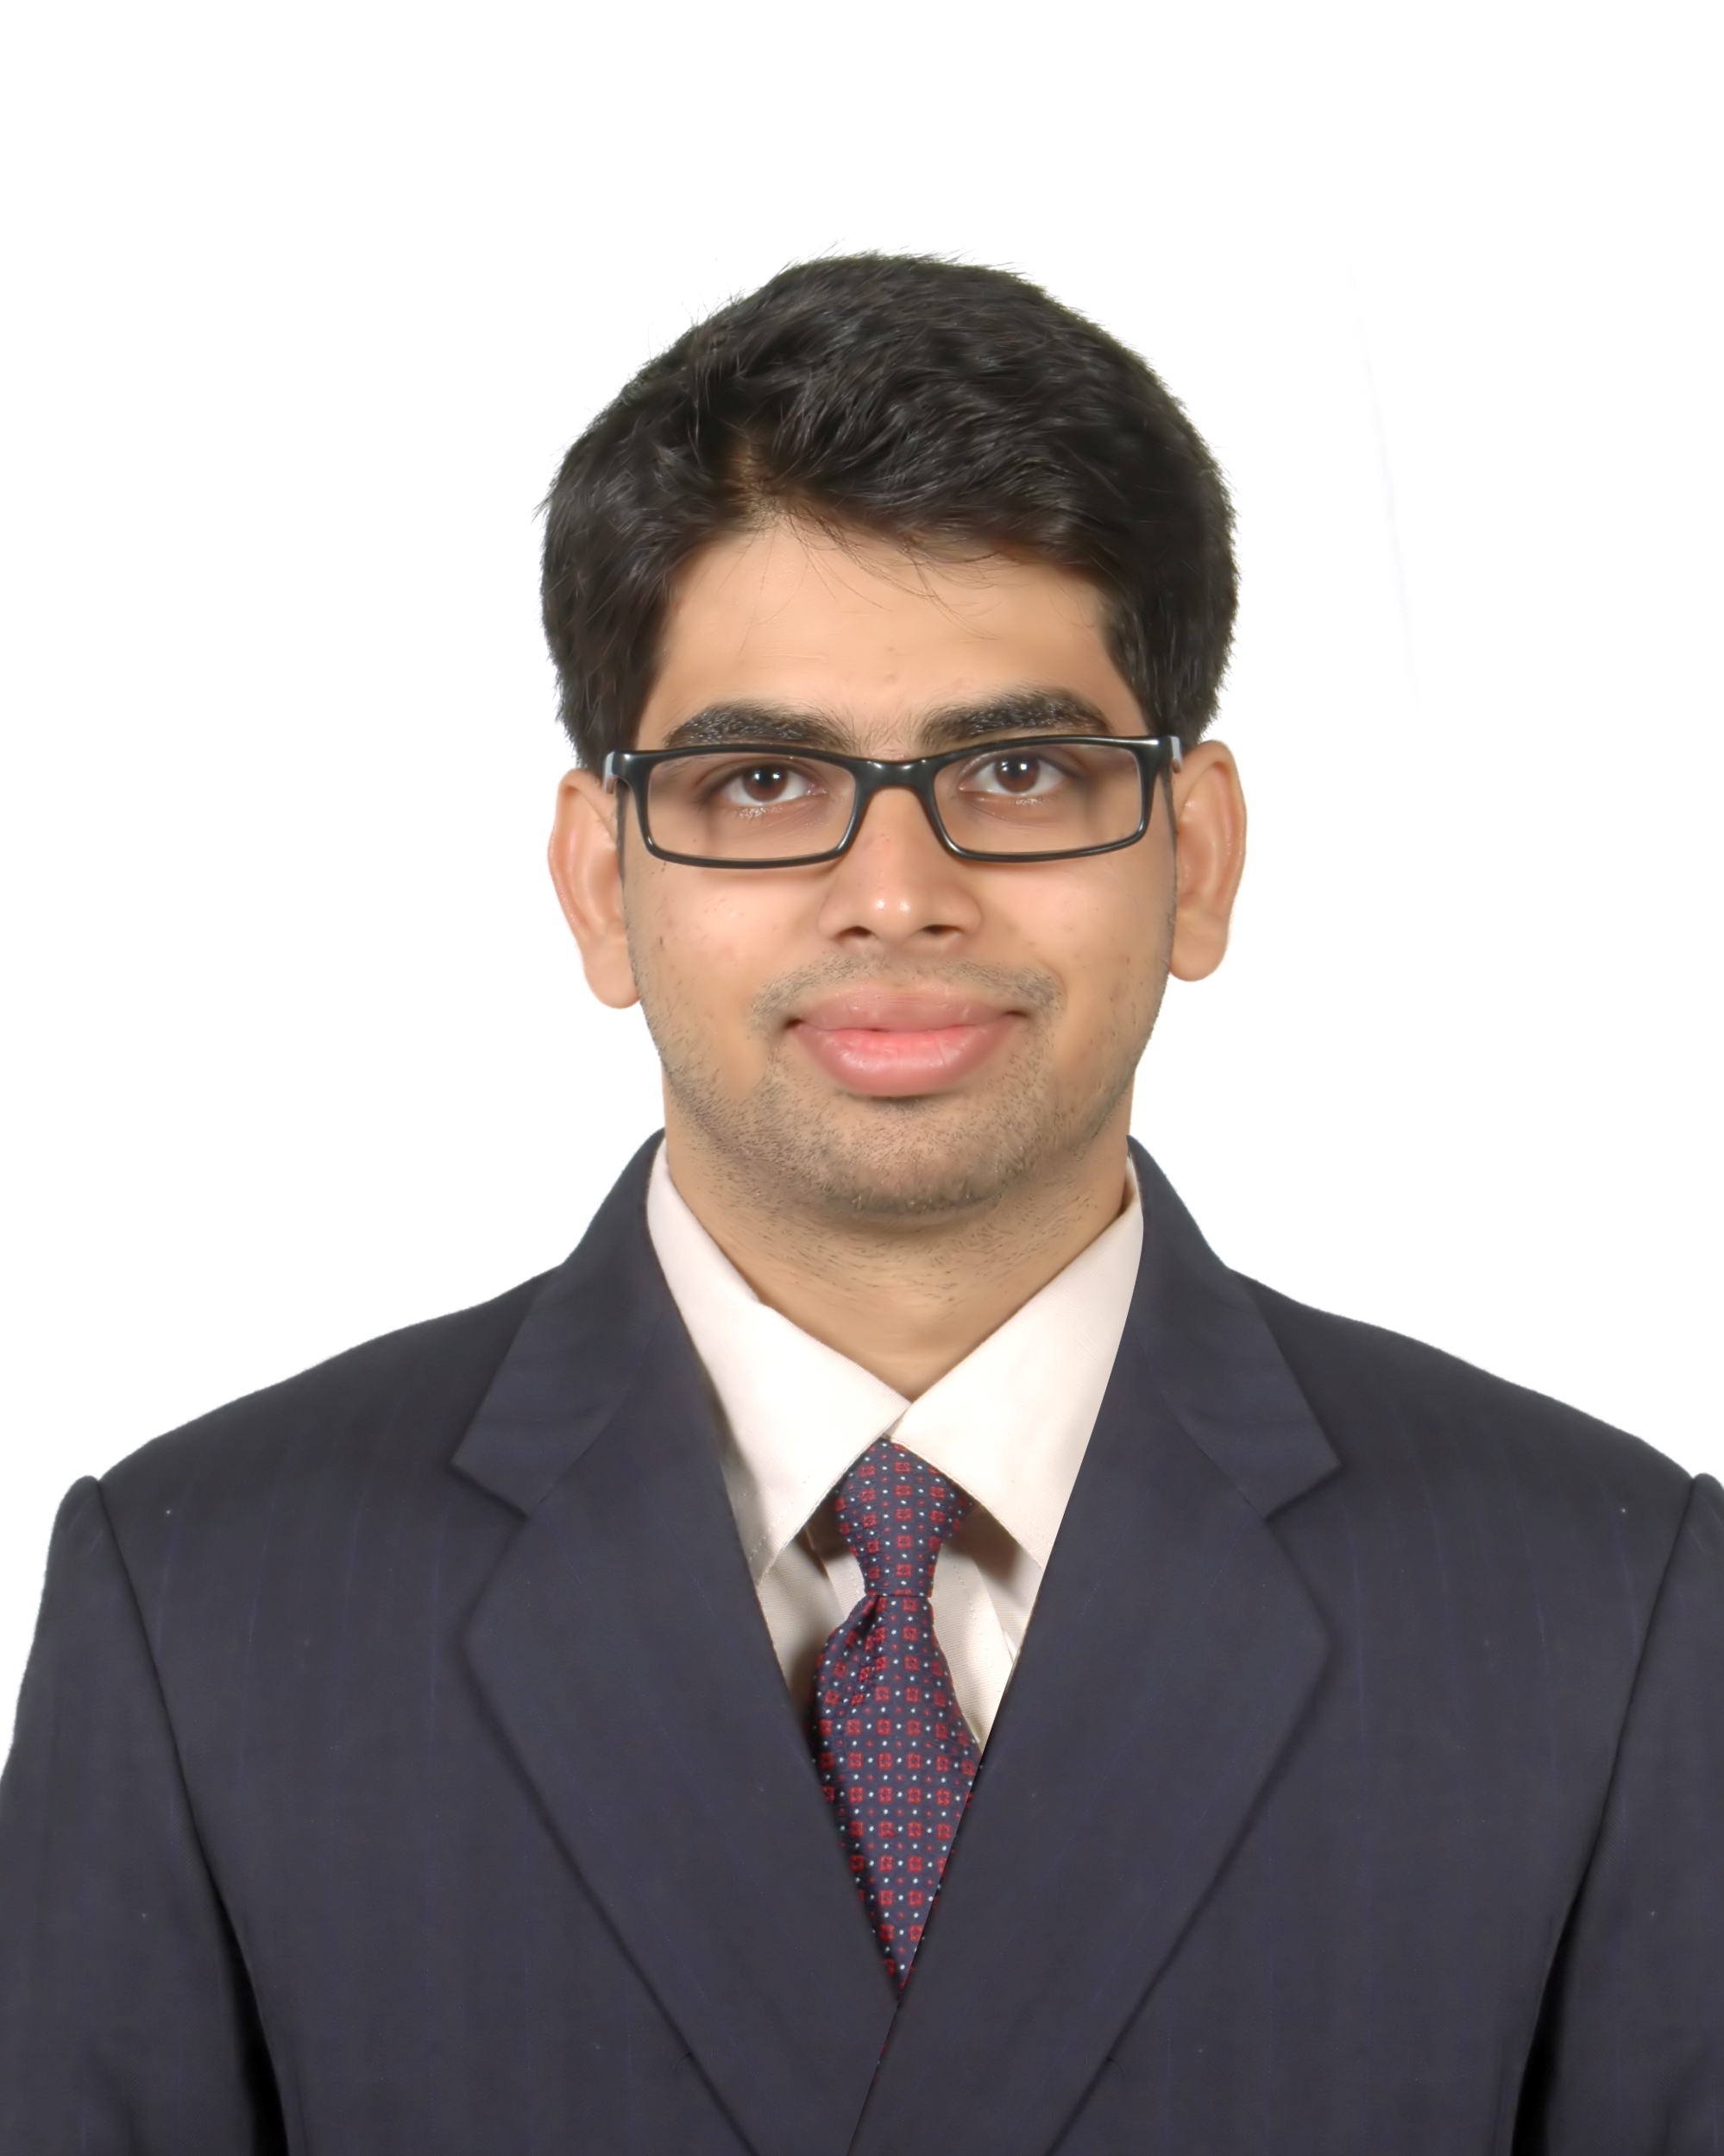
\includegraphics[scale=0.38]{DSC_6547.JPG}}\\
  & \\
%-----------------------------------------------------------  
  \textbf{\huge Amit M Girimaji }  \\
Email : amitgirimaji@gmail.com\\
Phone : 98864 27492 \\ 
'Sagar Nilaya', \\
3rd Cross, 2nd Stage, \\
Link Road, Ashok Nagar,\\
Shimoga 577201, \\
Karnataka \\
\end{tabular*}


%---------------------------------------------------------------

%%%%%%%%%%%%%%%%%%%%%%%%%%%%%%
\resheading{ Career Objective }
%%%%%%%%%%%%%%%%%%%%%%%%%%%%%%
\\
To obtain a challenging position in a high-quality engineering environment where my resourceful experience and academic skills will add value to organizational operations.  

%%%%%%%%%%%%%%%%%%%%%%%%%%%%%%
\resheading{Education}
%%%%%%%%%%%%%%%%%%%%%%%%%%%%%%

\begin{table}[h!]
	\centering
	
	\begin{tabular}{|c|c|c|c|c|c|}
		\hline
		Degree                                            & College / School                                                                                        & \begin{tabular}[c]{@{}c@{}}University \\ / Board\end{tabular}       & Pass \%                                                      & \begin{tabular}[c]{@{}c@{}}Passing \\ Year\end{tabular} & Remarks                                                                        \\ \hline
		\begin{tabular}[c]{@{}c@{}}B.E\\ ECE\end{tabular} & \begin{tabular}[c]{@{}c@{}}Jawaharlal Nehru National\\  College,of Engineering,\\  Shimoga\end{tabular} & VTU                                                                 & \begin{tabular}[c]{@{}c@{}}82.14\\ upto 6th Sem\end{tabular} & 2017                                                    & \begin{tabular}[c]{@{}c@{}}Tooper in\\ 1st and 3rd \\ semester\end{tabular}    \\ \hline
		PUC                                               & \begin{tabular}[c]{@{}c@{}}Sri Adichunchanagiri\\ Independent PU College,\\ Shimoga\end{tabular}        & \begin{tabular}[c]{@{}c@{}}Karnataka \\ State \\ Board\end{tabular} & 96.5                                                         & 2013                                                    & \begin{tabular}[c]{@{}c@{}}CET,Rank- 468\\ 1st Rank\\  in college\end{tabular} \\ \hline
		SSLC                                              & \begin{tabular}[c]{@{}c@{}}Sri Adichunchanagiri\\ Composite High School,\\ Shimoga\end{tabular}         & \begin{tabular}[c]{@{}c@{}}Karnataka\\ State\\ Board\end{tabular}   & 95.2                                                         & 2011                                                    &                                                                                \\ \hline
	\end{tabular}
\end{table}




%%%%%%%%%%%%%%%%%%%%%%%%%%%%%%
\resheading{Projects}
%%%%%%%%%%%%%%%%%%%%%%%%%%%%%%

\begin{enumerate}
	\item \textbf{'2-Wheeled Self-Balancing Robot with Joystick Control'} Got 4th place in eYRC 2016
	\item \textbf{Search and Rescue of Survivors during earthquake} Got 5th place in eYRC 2015
	\item C-Program: Account login control with special admin access along with 4 Prime number operations (2012)
\end{enumerate}



%%%%%%%%%%%%%%%%%%%%%%%%%%%%%%
\resheading{Hobby Projects}
%%%%%%%%%%%%%%%%%%%%%%%%%%%%%%

\begin{enumerate}
	\item Automated Train Level Crossing Indicator: got \textbf{2nd place} in hobby project exhibition 2015.
	\item Robot motion control using MATLAB image processing.
	\item Armed Robot for Dead Metal-Robo Wars.
\end{enumerate}

%%%%%%%%%%%%%%%%%%%%%%%%%%%%%%
\resheading{Internships}
%%%%%%%%%%%%%%%%%%%%%%%%%%%%%%

\begin{itemize} 
	\item Company:\hspace{1.4cm} \textbf{Rooftop Sundays} (Oct 2014 – Jun 2015) \\
	Role of Internship :   Social media marketing - To reach certain number of people daily in SoundCloud.
	\item Company:\hspace{1.4cm} \textbf{Band - Camp Mobiles} (Dec 2014 – Jan 2015) \\
	Role of Internship : To promote a mobile app ‘Band’ by creating a group and maintain it.
\end{itemize}



%%%%%%%%%%%%%%%%%%%%%%%%%%%%%%
\resheading{Trainings and Workshops}
%%%%%%%%%%%%%%%%%%%%%%%%%%%%%%

\begin{itemize}
	\item MSP-430 Micro-controller and Robotics Workshop - 2015
	\item 555 Timer and its Applications - 2015
	\item Soldering Techniques and Circuit Design using 555 Timer - 2014
	\item DST-Inspire Internship Camp - 2011
\end{itemize}


%%%%%%%%%%%%%%%%%%%%%%%%%%%%%%
\resheading{Technical Skills}
%%%%%%%%%%%%%%%%%%%%%%%%%%%%%%

\begin{itemize}
	\item Languages - C, C++, Embedded C/C++, Assembly (8051,8086)
	\item Hardware - MSP430, Atmega 2560, Arduino
	\item Tools - MATLAB,Scilab, Atmel Studio, Cadence Virtuoso
	\item Analog and Digital Circuit Design
	\item Adobe Photoshop, Adobe Auditon
\end{itemize}

%%%%%%%%%%%%%%%%%%%%%%%%%%%%%%
\resheading{Soft Skills}
%%%%%%%%%%%%%%%%%%%%%%%%%%%%%%

\begin{enumerate}
	\item Adaptability and flexibility
	\item Leadership
	\item Teamwork and collaboration
	\item Listening
	\item Presentation
	
\end{enumerate}


%%%%%%%%%%%%%%%%%%%%%%%%%%%%%%
\resheading{Extra Curricular Activities}
%%%%%%%%%%%%%%%%%%%%%%%%%%%%%%

\begin{itemize}
	\item \textbf{Black Belt} in Karate and \textbf{4 National Level participations with 1 Bronze Medal} in Muay Thai, Wushu and Karate games
	\item Invited as \textbf{Judge} for high school Science Project Exhibition        in Nov 2016.
	\item \textbf{Coordinated and Organized 3 Events:} Photography-2014, Technical Quiz-2015 and Mr. \& Ms. Techzone-2016 
	\item Organized \textbf{4 Basic Electronics Workshop} for Engineering and High School students.
	\item Secured \textbf{1st place in Photography} contest during Janvey 2014.

	
\end{itemize}

%%%%%%%%%%%%%%%%%%%%%%%%%%%%%%
\resheading{ Co-Curricular Activities }
%%%%%%%%%%%%%%%%%%%%%%%%%%%%%%

\begin{enumerate}
	\item Selected up to \textbf{3rd Round-Top 25} in India in \textbf{Enginx 2016 IOT Challenge by TCS} titled \textit{'Monitoring of Bedsore in Bedridden Patients Using IOT'.}
	
	\item Secured \textbf{1st place (2016) and 2nd place (2015)} in Circutrix, a \textbf{circuit design competition} held during National level event Techzone.

	\item \textbf{Presented Paper and secured 3rd place}, titled \textit{'Smart Borewell Rescue system using Embedded Technology'} in national level Techzone 2016.

	\item Secured \textbf{2nd place in Circuit Debugging} competition held during Spectrum-2015 under IETE.

	\item Secured \textbf{3rd place in C- Hunt}, a C-Programming contest held during Techzone-2014.
	
\end{enumerate}


%%%%%%%%%%%%%%%%%%%%%%%%%%%%%%
\resheading{ Personal Details }
%%%%%%%%%%%%%%%%%%%%%%%%%%%%%%
\\
Father’s Name: \hspace{0.5cm} D Mohan Girimaji\\
Mother’s Name: \hspace{0.45cm}Vani Girimaji   \\
Sex: 		   \hspace{2.3cm}Male            \\
Date of Birth: \hspace{0.8cm}26 - 06 -1995   \\
Nationality: 	\hspace{1.15cm}Indian          \\
Marital Status: \hspace{0.7cm}Single          \\



%%%%%%%%%%%%%%%%%%%%%%%%%%%%%%
\resheading{ References }
%%%%%%%%%%%%%%%%%%%%%%%%%%%%%%
\\
\textbf{\large Dr.Manjunath P } \\
HOD, Dept. of Electronics and Communication Engineering, \\
Jawaharlal Nehru National College of Engineering, \\
Shimoga\\
Email: manjup.jnnce@gmail.com \\
Phone: +91 9964378365




\end{document}